\documentclass[12pt]{article}
\oddsidemargin -0.5in
\evensidemargin -0.5in
\textwidth 7.2in
\topmargin -0.5in
\textheight 8in
\flushbottom

\usepackage[authoryear,round]{natbib} %a package for formatting citations
\usepackage{amsmath} %a package for good looking equations and symbols
\usepackage{algorithm2e} %a package for typesetting algorithms
% \usepackage{caption} %a package for more complex captions for figures/tables/images
\usepackage{subcaption} %extension of the caption package
\usepackage{url} %embedded, clickable links
\usepackage{fullpage} %including this package changes the default margins to use more of the page
\usepackage{graphicx} %package for inline images
\usepackage[usenames]{xcolor} %for adding color text
\usepackage{enumitem} %for nested numbered lists (like in the questions section)
\usepackage{hyperref}
\setlist[description]{style=nextline}

% \usepackage{hyperref}
% \usepackage{amsfonts}

\newcommand{\nextproblem}{
	\vfill
	\pagebreak
}
\setlist[itemize]{noitemsep, topsep=1pt}
\graphicspath{{plots/}}

\title{CS 4641 Machine Learning \\ Name Redacted | Section B Final Report}
\date{}
\author{}

\begin{document}

\maketitle

\section{Introduction to Dataset}
\subsection{\href{https://www.kaggle.com/insiyeah/musicfeatures}{Music Features from Kaggle} ($\leftarrow$ link)}
Every year I look forward to Spotify's end of year wrap up. As a consumer of sounds, I love seeing which "conventional categories," AKA genres, of music I sink thousands of hours in. This past year a new one made itself to the top of my list: Cpop. After some research, that stands for Chinese Pop. I've literally never heard of songs being labeled in this kind of genre before which led me to wonder how can someone categorize all the various kinds of music in the world. 
\\ \\
\textbf{TODO: Feature description.}
When I found this dataset, I was already interested in seeing if machine learning could analyze the sound waves of a piece of music and determine it's genre. However, that seems a too big of a computational task so I decided to use the features that are provided by this dataset. This dataset contains \textbf{1,000 datapoints} with \textbf{30 features per datapoint}. To prove that the features describe a piece pretty well, here are some of the features:
\begin{itemize}
    \item tempo: speed at which a passage of music is played
    \item beats: basic unit of time. Think about it as the rhythm you would tap your foot to when listening to a piece
    \item chroma\_stft: The Short Time Fourier Transform can be used to determine the sinusoidal frequency and phase content of local sections of a signal as it changes overtime (kind of like those visualizers that jump up and down)
    \item 20 mel-frequency ceptral coefficients that make up a mel-frequency cepstrum: representation of the short term power spectrum of a sound
\end{itemize}

\subsection{Supervised Learning Problem}
The underlying supervised learning problem is to \textbf{classify the genre} of pieces of music using the features of it's waveform. This dataset is \textbf{not trivial}. At first glance, there is no feature that determines the genre of a song trivially. To prove the non-triviality of this dataset, I tried to fit the centered data using sklearn.svm.LinearSVC (with a one-vs-the-rest multiclass scheme) 100 times and averaged the results.
\begin{itemize}
    \item avg testing accuracy: 0.62
    \item avg training accuracy: 0.71
\end{itemize}
The training accuracy is not high enough to prove that the dataset is linearly separable. But to further research the triviality of the dataset, I did a few more experiements:
\begin{itemize}
    \item 3D PCA Plot
    \\ 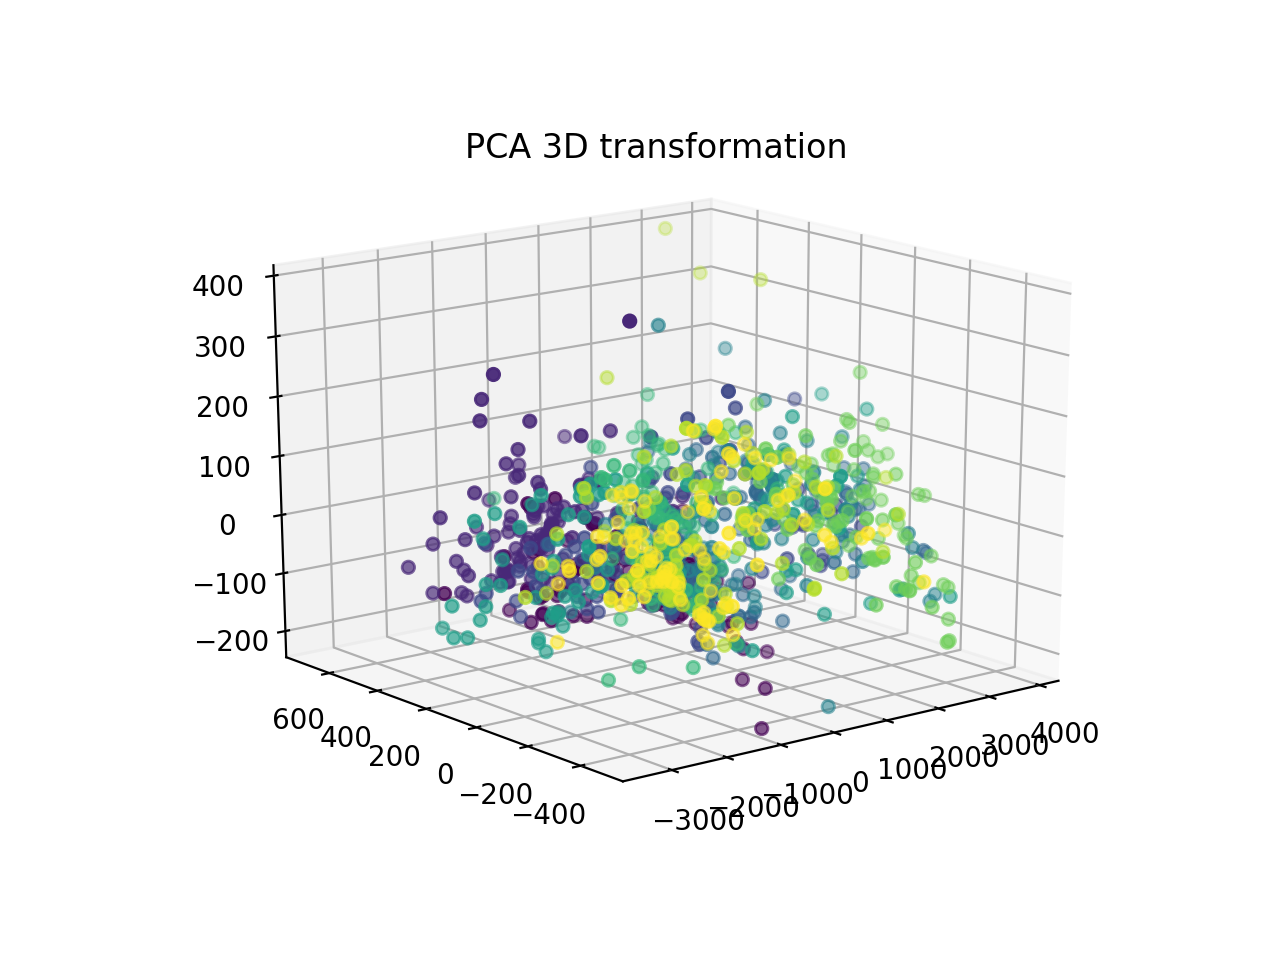
\includegraphics[width=0.45\textwidth]{pca0} 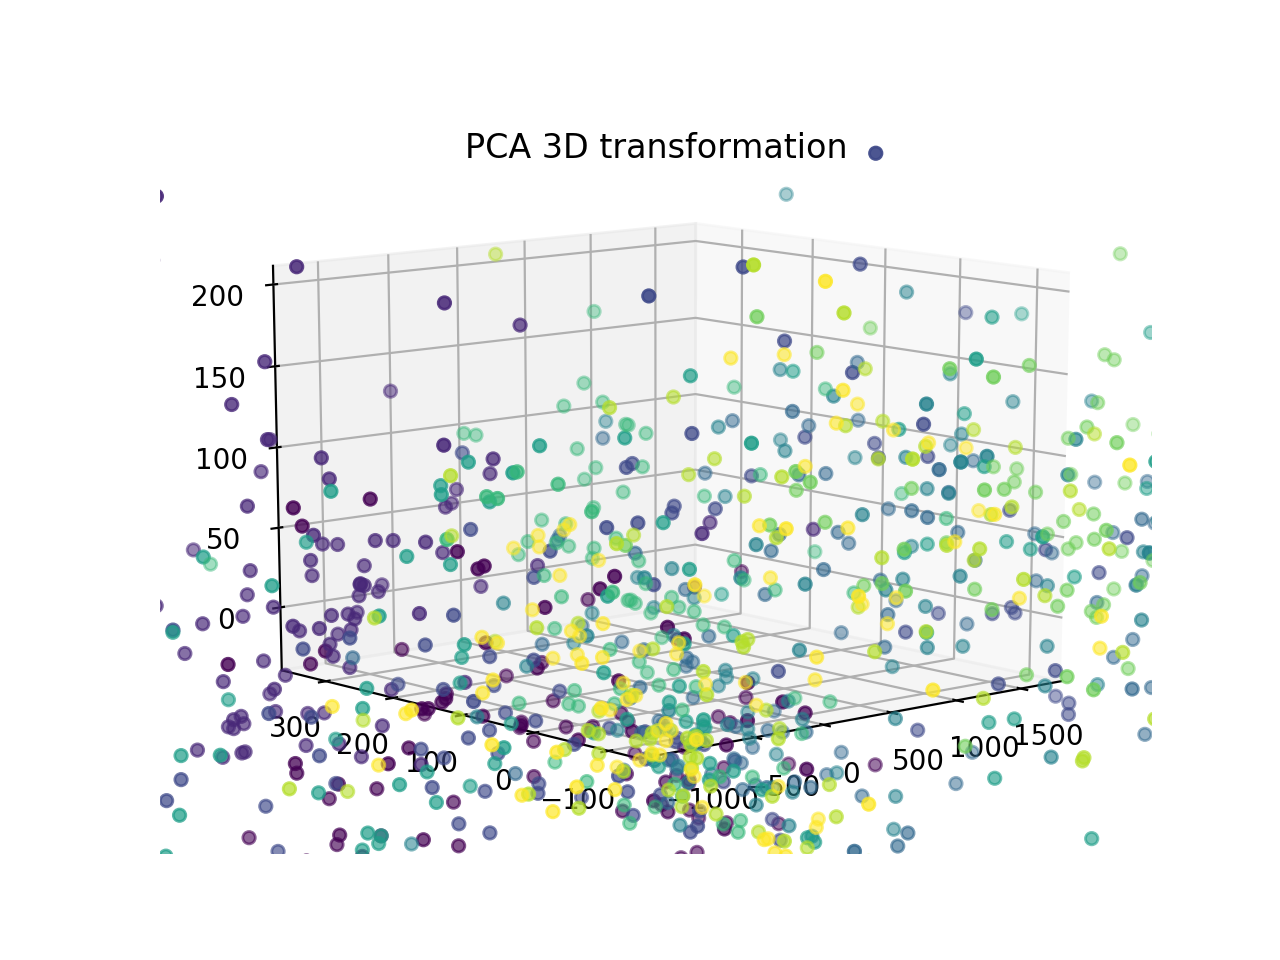
\includegraphics[width=0.45\textwidth]{pca1}
    \\ The graph on the right is a zoomed in version of the left graph. It is clear that there are many data points mixed together and the dataset is at least not linearly separable in 3 dimensions.
    \item Linear Regression: I one-hot-encoded the labels and tried to fit a linear regression. The testing and training accuracy was 0.26 and 0.31 respectively. This serves as more evidence that the dataset is non-trivial.
\end{itemize}
After these additional experiements, I have convinced myself that my \textbf{dataset is non-trivial}.

\subsection{Performance Metrics}
I will be using \textbf{Nested 2-Folds Cross Validation} for hyperparameter tuning. In Nested 2-Folds Cross Validation, I will split data randomly into two halves, X and Y. Then I will perform 10-Folds Cross Validation on X to tune for optimal hyperparameters. I'll be using sklearn's GridSearchCV for hyperparameter tuning. Then I will take the hyper parameters tuned from X and score it using 10-folds cross validation on Y. Then I will switch X and Y and repeat the process. Here is a step by step:
\begin{enumerate}
    \item Split dataset into X and Y
    \item 10 folds cross validation on X and tune hyperparameters
    \item Use hyperparameters from 2. to create classfier C
    \item Split Y into 10 folds. For each fold i: train C on all other folds and score on current fold i. This gives 10 scores
    \item Switch X and Y and repeat steps 1 to 4. This gives 20 scores in total
    \item Use the 20 scores to calculate confidence interval for the classifier
\end{enumerate}
I also plan on analyzing the \textbf{confusion matrix} of resulting test accuracies for each learning method and using \textbf{confidence intervals} as a means of comparing learning methods.

\section{Description of Algorithms}
\subsection{Random Forests with Bagging}
A random forest consists of a large number of individual decision trees that form an ensemble. An ensemble bascially uses multiple algorithms to obtain more accurate predictions than any one individual of the ensemble. In a random forest, the ensemble is made up of relatively uncorrelated decision trees. Bagging (Bootstrap Aggregation) is a method that allows each decision tree in the random forest to randomly sample the dataset with replacement. Since decision trees are very sensitive the training data, this greatly increases the variablility of the decision trees. Here are the hyperparameters I will optimize:
\begin{itemize}
    \item n\_estimators: [100, 200, 300, 400, 500]
    \\ Number of trees in the forest. Affects the size of the random forest.
    \item max\_depth: [100, 200, 300, 400, 500]
    \\ The maximum depth of each decision tree. affects the complexity of each tree.
    \item max\_features: ['sqrt', 'log2', None]
    \\ The max size of the random subsets of features to consider when splitting a node.
\end{itemize}

\subsection{Support Vector Machines with a non-linear kernel}
SVMs attempts to separate datapoints by its labels by finding the best hyperplane using the large margin principle. For non-linear data, it can use the kernel trick to map the data to a higher dimension in hopes of finding a more suitable hyperplane. However, SVMs are inherently binary classifiers so it is not suitable for my dataset that has 10 unique labels. I will be using the \textbf{one-versus-all} classification technique to train my multiclass SVM. Here are the hyperparameters I will optimize:
\begin{itemize}
    \item C: [1.e-02, 1.e-01, 1.e+00, 1.e+01, 1.e+02, 1.e+03, 1.e+04]
    \\ Regularization paramenter represents how much I want to avoid misclassifying each training example. Large C will choose the a plane that correctly classifies the most training examples. Small C will choose a plane with a larger margin even if that plane wrongly classifies more training examples
    \item kernel: ['poly', 'rbf', 'sigmoid'] 
    \\ The kernel type to use when mapping the data to a new dimension space. This will affect the separablility of the data after it is mapped to a new dimension.
    \item gamma: [1.e-03, 1.e-02, 1.e-01, 1.e+00, 1.e+01, 1.e+02, 1.e+03]
    \\ Kernel coefficient for rbf, poly, and sigmoid.
\end{itemize}

\subsection{Neural Network}
A neural net is basically a bunch of algorithms, designed and modeled loosely like a human brain, that can \textbf{recognize patterns}. They all start with an input layer, which can be thought of an array of inputs such as numbers, rgb values, words, etc. The input layer is \textbf{densely connected} to the first hidden layer and the first hidden layer to the next hidden layer. There can be many hidden layers and each layer is made up of some amount of neurons. Each neuron's job is to compute a \textbf{weighted average} of its input, and this sum is passed through a non-linear activation function such as a sigmoid or ReLU. Eventually the last hidden layer will connect to an output layer responsible for outputting the prediction. The entire neural net is trained using a technique called \textbf{back propagation}, which calculates a gradient descent to nudge the weights for a perceptron towards its theoretical optimal value. Here are the hyperparameters I will optimize for my nerual net:
\begin{itemize}
    \item hidden\_layer\_sizes: [ (10, 10, 10), (20, 20, 20), (10, 10), (20, 20) ]
    \\ A tuple of length (number of layers - 2) where the element at position i represents the number of neurons in hidden layer i.
    \item activation: ['identity', 'logistic', 'tanh', 'relu']
    \\ The activation function for the hidden layer.
    \item solver: ['lbfgs', 'sgd', 'adam']
    \\ The solver for weight optimization for each neuron
    \item apha: [0.0001, 0.001]
    \\ The L2 regularization penalty parameter. This penalizes larger weight values to favor smaller values in the weight matrix. This in turn decreases the effect of the activation function, resulting in a less complex function. We want a less complex function to avoid overfitting
    \item learning\_rate\_init: [0.01, 0.001]
    \\ For my purposes, this will be the learning rate for the entirety of the training because I will be using a constant learning rate for all trials to limit the complexity of this GridSearch.
    \item max\_iter: [500, 1000]
    \\ The limit on the number of iterations of training. The solver iterates until convergence or when it has reach the max number of iterations.
\end{itemize}

\nextproblem

\href{https://www.quora.com/What-are-C-and-gamma-with-regards-to-a-support-vector-machine}{1} \\
\href{https://scikit-learn.org/stable/auto_examples/svm/plot_rbf_parameters.html}{2} \\
\href{https://machinelearningmastery.com/save-load-machine-learning-models-python-scikit-learn/}{3} \\



\end{document}

